% Graphic for TeX using PGF
% Title: /home/satenske/cours/AP/tad2/TD9/1-1.dia
% Creator: Dia v0.97.1
% CreationDate: Tue May 24 08:21:25 2011
% For: satenske
% \usepackage{tikz}
% The following commands are not supported in PSTricks at present
% We define them conditionally, so when they are implemented,
% this pgf file will use them.
\ifx\du\undefined
  \newlength{\du}
\fi
\setlength{\du}{15\unitlength}
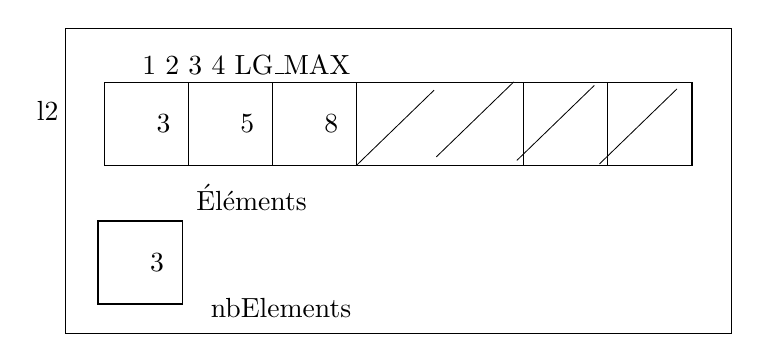
\begin{tikzpicture}
\pgftransformxscale{1.000000}
\pgftransformyscale{-1.000000}
\definecolor{dialinecolor}{rgb}{0.000000, 0.000000, 0.000000}
\pgfsetstrokecolor{dialinecolor}
\definecolor{dialinecolor}{rgb}{1.000000, 1.000000, 1.000000}
\pgfsetfillcolor{dialinecolor}
\pgfsetlinewidth{0.030000\du}
\pgfsetdash{}{0pt}
\pgfsetdash{}{0pt}
\pgfsetmiterjoin
\definecolor{dialinecolor}{rgb}{1.000000, 1.000000, 1.000000}
\pgfsetfillcolor{dialinecolor}
\fill (5.250000\du,4.800000\du)--(5.250000\du,12.150000\du)--(21.300000\du,12.150000\du)--(21.300000\du,4.800000\du)--cycle;
\definecolor{dialinecolor}{rgb}{0.000000, 0.000000, 0.000000}
\pgfsetstrokecolor{dialinecolor}
\draw (5.250000\du,4.800000\du)--(5.250000\du,12.150000\du)--(21.300000\du,12.150000\du)--(21.300000\du,4.800000\du)--cycle;
\pgfsetlinewidth{0.030000\du}
\pgfsetdash{}{0pt}
\pgfsetdash{}{0pt}
\pgfsetmiterjoin
\definecolor{dialinecolor}{rgb}{1.000000, 1.000000, 1.000000}
\pgfsetfillcolor{dialinecolor}
\fill (6.200000\du,6.100000\du)--(6.200000\du,8.100000\du)--(20.364675\du,8.100000\du)--(20.364675\du,6.100000\du)--cycle;
\definecolor{dialinecolor}{rgb}{0.000000, 0.000000, 0.000000}
\pgfsetstrokecolor{dialinecolor}
\draw (6.200000\du,6.100000\du)--(6.200000\du,8.100000\du)--(20.364675\du,8.100000\du)--(20.364675\du,6.100000\du)--cycle;
\pgfsetlinewidth{0.030000\du}
\pgfsetdash{}{0pt}
\pgfsetdash{}{0pt}
\pgfsetmiterjoin
\definecolor{dialinecolor}{rgb}{1.000000, 1.000000, 1.000000}
\pgfsetfillcolor{dialinecolor}
\fill (6.200000\du,6.100000\du)--(6.200000\du,8.100000\du)--(8.231000\du,8.100000\du)--(8.231000\du,6.100000\du)--cycle;
\definecolor{dialinecolor}{rgb}{0.000000, 0.000000, 0.000000}
\pgfsetstrokecolor{dialinecolor}
\draw (6.200000\du,6.100000\du)--(6.200000\du,8.100000\du)--(8.231000\du,8.100000\du)--(8.231000\du,6.100000\du)--cycle;
\pgfsetlinewidth{0.030000\du}
\pgfsetdash{}{0pt}
\pgfsetdash{}{0pt}
\pgfsetmiterjoin
\definecolor{dialinecolor}{rgb}{1.000000, 1.000000, 1.000000}
\pgfsetfillcolor{dialinecolor}
\fill (8.216000\du,6.101250\du)--(8.216000\du,8.101250\du)--(10.247000\du,8.101250\du)--(10.247000\du,6.101250\du)--cycle;
\definecolor{dialinecolor}{rgb}{0.000000, 0.000000, 0.000000}
\pgfsetstrokecolor{dialinecolor}
\draw (8.216000\du,6.101250\du)--(8.216000\du,8.101250\du)--(10.247000\du,8.101250\du)--(10.247000\du,6.101250\du)--cycle;
\pgfsetlinewidth{0.030000\du}
\pgfsetdash{}{0pt}
\pgfsetdash{}{0pt}
\pgfsetmiterjoin
\definecolor{dialinecolor}{rgb}{1.000000, 1.000000, 1.000000}
\pgfsetfillcolor{dialinecolor}
\fill (10.237250\du,6.098750\du)--(10.237250\du,8.098750\du)--(12.268250\du,8.098750\du)--(12.268250\du,6.098750\du)--cycle;
\definecolor{dialinecolor}{rgb}{0.000000, 0.000000, 0.000000}
\pgfsetstrokecolor{dialinecolor}
\draw (10.237250\du,6.098750\du)--(10.237250\du,8.098750\du)--(12.268250\du,8.098750\du)--(12.268250\du,6.098750\du)--cycle;
\pgfsetlinewidth{0.030000\du}
\pgfsetdash{}{0pt}
\pgfsetdash{}{0pt}
\pgfsetmiterjoin
\definecolor{dialinecolor}{rgb}{1.000000, 1.000000, 1.000000}
\pgfsetfillcolor{dialinecolor}
\fill (16.296075\du,6.102187\du)--(16.296075\du,8.102187\du)--(18.327075\du,8.102187\du)--(18.327075\du,6.102187\du)--cycle;
\definecolor{dialinecolor}{rgb}{0.000000, 0.000000, 0.000000}
\pgfsetstrokecolor{dialinecolor}
\draw (16.296075\du,6.102187\du)--(16.296075\du,8.102187\du)--(18.327075\du,8.102187\du)--(18.327075\du,6.102187\du)--cycle;
\pgfsetlinewidth{0.030000\du}
\pgfsetdash{}{0pt}
\pgfsetdash{}{0pt}
\pgfsetmiterjoin
\definecolor{dialinecolor}{rgb}{1.000000, 1.000000, 1.000000}
\pgfsetfillcolor{dialinecolor}
\fill (18.317325\du,6.099687\du)--(18.317325\du,8.099687\du)--(20.348325\du,8.099687\du)--(20.348325\du,6.099687\du)--cycle;
\definecolor{dialinecolor}{rgb}{0.000000, 0.000000, 0.000000}
\pgfsetstrokecolor{dialinecolor}
\draw (18.317325\du,6.099687\du)--(18.317325\du,8.099687\du)--(20.348325\du,8.099687\du)--(20.348325\du,6.099687\du)--cycle;
\pgfsetlinewidth{0.030000\du}
\pgfsetdash{}{0pt}
\pgfsetdash{}{0pt}
\pgfsetmiterjoin
\definecolor{dialinecolor}{rgb}{1.000000, 1.000000, 1.000000}
\pgfsetfillcolor{dialinecolor}
\fill (6.040000\du,9.441250\du)--(6.040000\du,11.441250\du)--(8.071000\du,11.441250\du)--(8.071000\du,9.441250\du)--cycle;
\definecolor{dialinecolor}{rgb}{0.000000, 0.000000, 0.000000}
\pgfsetstrokecolor{dialinecolor}
\draw (6.040000\du,9.441250\du)--(6.040000\du,11.441250\du)--(8.071000\du,11.441250\du)--(8.071000\du,9.441250\du)--cycle;
% setfont left to latex
\definecolor{dialinecolor}{rgb}{0.000000, 0.000000, 0.000000}
\pgfsetstrokecolor{dialinecolor}
\node[anchor=west] at (7.055500\du,10.441250\du){3};
% setfont left to latex
\definecolor{dialinecolor}{rgb}{0.000000, 0.000000, 0.000000}
\pgfsetstrokecolor{dialinecolor}
\node[anchor=west] at (7.215500\du,7.100000\du){3};
% setfont left to latex
\definecolor{dialinecolor}{rgb}{0.000000, 0.000000, 0.000000}
\pgfsetstrokecolor{dialinecolor}
\node[anchor=west] at (9.231500\du,7.101250\du){5};
% setfont left to latex
\definecolor{dialinecolor}{rgb}{0.000000, 0.000000, 0.000000}
\pgfsetstrokecolor{dialinecolor}
\node[anchor=west] at (11.252750\du,7.098750\du){8};
\pgfsetlinewidth{0.020000\du}
\pgfsetdash{}{0pt}
\pgfsetdash{}{0pt}
\pgfsetbuttcap
{
\definecolor{dialinecolor}{rgb}{0.000000, 0.000000, 0.000000}
\pgfsetfillcolor{dialinecolor}
% was here!!!
\definecolor{dialinecolor}{rgb}{0.000000, 0.000000, 0.000000}
\pgfsetstrokecolor{dialinecolor}
\draw (12.268250\du,8.098750\du)--(14.135000\du,6.291250\du);
}
\pgfsetlinewidth{0.020000\du}
\pgfsetdash{}{0pt}
\pgfsetdash{}{0pt}
\pgfsetbuttcap
{
\definecolor{dialinecolor}{rgb}{0.000000, 0.000000, 0.000000}
\pgfsetfillcolor{dialinecolor}
% was here!!!
\definecolor{dialinecolor}{rgb}{0.000000, 0.000000, 0.000000}
\pgfsetstrokecolor{dialinecolor}
\draw (14.189140\du,7.897890\du)--(16.055890\du,6.090390\du);
}
\pgfsetlinewidth{0.020000\du}
\pgfsetdash{}{0pt}
\pgfsetdash{}{0pt}
\pgfsetbuttcap
{
\definecolor{dialinecolor}{rgb}{0.000000, 0.000000, 0.000000}
\pgfsetfillcolor{dialinecolor}
% was here!!!
\definecolor{dialinecolor}{rgb}{0.000000, 0.000000, 0.000000}
\pgfsetstrokecolor{dialinecolor}
\draw (16.129140\du,7.982890\du)--(17.995890\du,6.175390\du);
}
\pgfsetlinewidth{0.020000\du}
\pgfsetdash{}{0pt}
\pgfsetdash{}{0pt}
\pgfsetbuttcap
{
\definecolor{dialinecolor}{rgb}{0.000000, 0.000000, 0.000000}
\pgfsetfillcolor{dialinecolor}
% was here!!!
\definecolor{dialinecolor}{rgb}{0.000000, 0.000000, 0.000000}
\pgfsetstrokecolor{dialinecolor}
\draw (18.119140\du,8.067890\du)--(19.985890\du,6.260390\du);
}
% setfont left to latex
\definecolor{dialinecolor}{rgb}{0.000000, 0.000000, 0.000000}
\pgfsetstrokecolor{dialinecolor}
\node[anchor=west] at (8.175000\du,8.875000\du){Éléments};
% setfont left to latex
\definecolor{dialinecolor}{rgb}{0.000000, 0.000000, 0.000000}
\pgfsetstrokecolor{dialinecolor}
\node[anchor=west] at (8.525000\du,11.525000\du){nbElements};
% setfont left to latex
\definecolor{dialinecolor}{rgb}{0.000000, 0.000000, 0.000000}
\pgfsetstrokecolor{dialinecolor}
\node[anchor=west] at (6.875000\du,5.675000\du){1       2       3     4                             LG\_MAX};
% setfont left to latex
\definecolor{dialinecolor}{rgb}{0.000000, 0.000000, 0.000000}
\pgfsetstrokecolor{dialinecolor}
\node[anchor=west] at (4.335000\du,6.791250\du){l2};
\end{tikzpicture}
